\documentclass[14pt,a4paper]{extarticle}
\usepackage[T2A]{fontenc}
\usepackage[utf8]{inputenc}
\usepackage[english,russian]{babel}
\usepackage{lmodern}
\usepackage{geometry}
\usepackage{array}
\usepackage{tabularx}
\usepackage{longtable}
\usepackage{ltablex}
\usepackage{booktabs}
\usepackage{hyperref}
\usepackage{indentfirst}
\usepackage{microtype}
\usepackage{graphicx}
\usepackage{setspace}
\usepackage{listings}
\usepackage{graphicx}
\usepackage{caption}
\usepackage{float}
\usepackage{tocloft}
\usepackage{titlesec}
\usepackage{newtxtext,newtxmath}
\usepackage{eqexpl}

\newcommand{\R}{\ensuremath{\mathbb{R}}}

\titleformat{\section}        % форматируем \section
  {\normalfont\bfseries}      % стиль: обычный + жирный
  {\thesection.}              % номер секции с точкой
  {2mm}                       % расстояние между номером и текстом
  {}                           % перед заголовком можно добавить что-то
\titlespacing*{\section}{1.5cm}{*3}{*1}  % {отступ слева}{отступ сверху}{отступ снизу}

\captionsetup{justification=centering}
\renewcommand{\ttdefault}{cmtt}
\keepXColumns
\setlength{\parindent}{3em}
\newgeometry{left=2.5cm,right=2.5cm,top=3cm,bottom=2.5cm}

\renewcommand{\contentsname}{\hspace*{4em}{\smallСодержание}}
\setlength{\cftbeforesecskip}{0.5em}
\renewcommand{\cftsecleader}{\cftdotfill{\cftdotsep}}
\renewcommand{\cftsecaftersnum}{.\hspace{2mm}}

\title{Отчёт по Машинному обучению}
\author{Выполнил студент группы М-РИТ-25-1, Станиславчук Сергей}

\begin{document}

\setstretch{1.5}
\noindent
\begin{minipage}[t]{0.01\textwidth}
    \includegraphics{~/programmer/++Programmer/5_1/LSTU.jpg}
\end{minipage}%
\begin{minipage}[c]{1.1\linewidth}
    \centering
    {\small
    МИНИСТЕРСТВО НАУКИ И ВЫСШЕГО ОБРАЗОВАНИЯ РФ \\[1em]
    ФЕДЕРАЛЬНОЕ ГОСУДАРСТВЕННОЕ БЮДЖЕТНОЕ \\
    ОБРАЗОВАТЕЛЬНОЕ УЧРЕЖДЕНИЕ ВЫСШЕГО ОБРАЗОВАНИЯ \\
    «ЛИПЕЦКИЙ ГОСУДАРСТВЕННЫЙ ТЕХНИЧЕСКИЙ УНИВЕРСИТЕТ»
    }
\end{minipage}%

\vspace{3em}

\noindent
\hspace{1em}%
\begin{minipage}[t]{0.8\textwidth}
\textbf{Институт} \hspace{2em} компьютерных наук \\
\textbf{Кафедра} \hspace{2em} автоматизированных систем управления
\end{minipage}

\vspace{6em}

\begin{center}
    Курсовая работа \\
    по дисциплине: <<Машинное обучение>> \\
    на тему: <<Атаки в системах машинного обучения>>
\end{center}

\vspace{6em}

\noindent
\begin{tabular*}{\textwidth}{@{\extracolsep{\fill}} l c r }
    Студент М-РИТ-25-1 & \makebox[4cm]{\hrulefill} & Станиславчук С.М. \\[2em]
Руководитель & \\
Доцент, д.т.н. & \makebox[4cm]{\hrulefill} & Сараев П.В. \\
\end{tabular*}

\vfill
\begin{center}
    Липецк, 2025
\end{center}

\thispagestyle{empty}

\newpage
\tableofcontents
\newpage

\section{Цель работы}

Реализовать и проанализировать модель машинного обучения, решающую задачу
классификации, а также исследовать её устойчивость к различным видам атак.

\section{Задание}
\begin{sloppypar}
    Выбранная тематика: 8. Атаки в системах машинного обучения.\\

    1. Подобрать интересующее соревнование и извлечь из него датасет \\
    \indent2. Написать программу, которая обучит модель на выбранном датасете \\
    \indent3. Провести анализ уязвимости полученной модели \\
    \indent4. Провести атаки на модель.\\
    \indent5. Сравнить атакованные и нетронутые результаты. \\
    \indent6. Предложить усиление слабых мест модели.\\
\end{sloppypar}

\newpage
\section{Исходный датасет}
    В качестве задания, был выбран датасет, использующийся в соревновании
    <<Titanic - Machine Learning from Disaster>> с сервиса $kaggle.com$, тематикой
    которого, как видно из названия, является крушение одноименного судна.

    Датасет включает в себя всех пассажиров "Титаника\", находящихся на нем в момент крушения.
    Задача соревнования: обучить модель таким образом, чтобы она могла определить по входным данным
    пассажира спасется он или нет в результате крушения.

\begin{enumerate}
    \setlength{\itemindent}{2em}
    \item \texttt{survival} — факт выживания (0 — нет, 1 — да)
    \item \texttt{pclass} — класс билета (1 — первый, 2 — второй, 3 — третий)
    \item \texttt{sex} — пол пассажира
    \item \texttt{age} — возраст
    \item \texttt{sibsp} — количество супругов и детей на борту
    \item \texttt{parch} — количество родителей и детей на борту
    \item \texttt{ticket} — номер билета
    \item \texttt{fare} — стоимость проезда
    \item \texttt{cabin} — номер каюты
    \item \texttt{embarked} — порт посадки
    (C — Шербур, Q — Квинстаун, S — Саутгемптон)
\end{enumerate}

    Пояснение к переменным: \\
    \indent pclass: показатель социально-экономического статуса
    \begin{itemize}
        \setlength{\itemindent}{2em}
        \item 1-й - Высший
        \item 2-й - Средний
        \item 3-й - Нижний
    \end{itemize}

    age: возраст указывается дробно, если он меньше 1.
    sibsp: набор данных определеяет семейные отношения следующим образом:
        Дети - брат, сестра, сводный брат, сводная сестра.
        Супруг - муж, жена

    parch: Набор данных определяет семейные отношения следующим образом:
        Родитель - мать, отец
        Ребенок - дочь, сын, падчерица, пасынок (Некоторые дети путешествовали
        только с няней, для них parch = 0) \\

    Датасет состоит из двух частей: train и test, оба в формате .csv.
    Файл train.csv состоит из 418 записей (пассажиров), test.csv из 891.

\section{Программа для обучения модели}

Так как модель следует обучить предугадыванию выживания, то возможны лишь два
исхода для пассажира: выживет или нет. Правильным решением для такой задачи
будет использование методов классификации для обучения модели. Всего будет 2
класса: выживший (1) и невыживший (0). Таким образом, задача является бинарной классификацией.

Для обучения модели была реализована программа на языке Python с использованием
библиотек \texttt{pandas}, \texttt{scikit-learn}, \texttt{numpy}, \texttt{joblib}.

\begin{itemize}
    \item \texttt{pandas} — для загрузки датасета, обработки пропущенных значений и преобразования признаков;
    \item \texttt{numpy} — для выполнения численных операций и работы с массивами данных;
    \item \texttt{scikit-learn} — для реализации алгоритмов машинного обучения, разбиения данных на обучающую и тестовую выборки, а также оценки качества модели;
    \item \texttt{joblib} — для сохранения и последующей загрузки обученной модели.
\end{itemize}

На первом этапе выполняется загрузка данных и их предварительная обработка.
Из датасета удаляются признаки, не оказывающие существенного влияния на результат
классификации (идентификаторы пассажиров, имена и номера билетов).
Пропущенные значения возраста заменяются медианным значением,
а отсутствующие данные о порте посадки — наиболее часто встречающимся значением.

Категориальные признаки, такие как пол пассажира и порт посадки, преобразуются
в числовой формат с использованием бинарного кодирования.
Информация о каюте дополнительно обрабатывается: из строкового значения
выделяется палуба и числовой номер каюты, что позволяет сохранить полезные
пространственные характеристики расположения пассажиров на судне.

В качестве модели классификации был выбран алгоритм \textit{Random Forest},
основанный на ансамбле решающих деревьев.
Данный алгоритм обладает устойчивостью к выбросам,
не требует масштабирования признаков и способен эффективно
обрабатывать нелинейные зависимости между входными данными.

Обучение модели производится на обучающей выборке с последующим разделением
данных на тренировочную и валидационную части.
Качество классификации оценивается с использованием метрик точности (Accuracy)
и площади под ROC-кривой (AUC). Результаты выполнения программы представлены на
рисунке \ref{fig:teach}.

\begin{figure}[H]
    \centering
    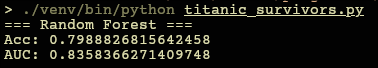
\includegraphics[width=0.78\textwidth]{pic1.png}
    \refstepcounter{figure}
    \caption*{Рисунок \thefigure\ — Результат выполнения обученной модели}
    \label{fig:teach}
\end{figure}

Как видно из рисунка, показатель точности достаточно высокий $\approx 0.7989$
Таким образом, определение класса для большинства объектов выборки прошло успешно.
А показатель AUC еще выше $\approx 0.8358$, что свидетельствует о высокой
способности модели различать пассажиров, выживших и погибших в результате крушения.
Как раз та самая точность, на которой будут заметны результаты атак.

\section{Анализ уязвимостей модели}

Несмотря на достаточно высокие значения метрик качества, модель машинного обучения
может обладать рядом уязвимостей, связанных с особенностями обучающего датасета,
предобработки данных и используемого алгоритма.

Под уязвимостью в данном случае понимается возможность искусственного изменения
входных данных таким образом, чтобы модель выдала неверный результат, либо
снижение устойчивости предсказаний при незначительных изменениях признаков.

Зависимость от ключевых признаков.

График самых влиятельных на результат признаков представлен на рисунке \ref{fig:important}.

\begin{figure}[H]
    \centering
    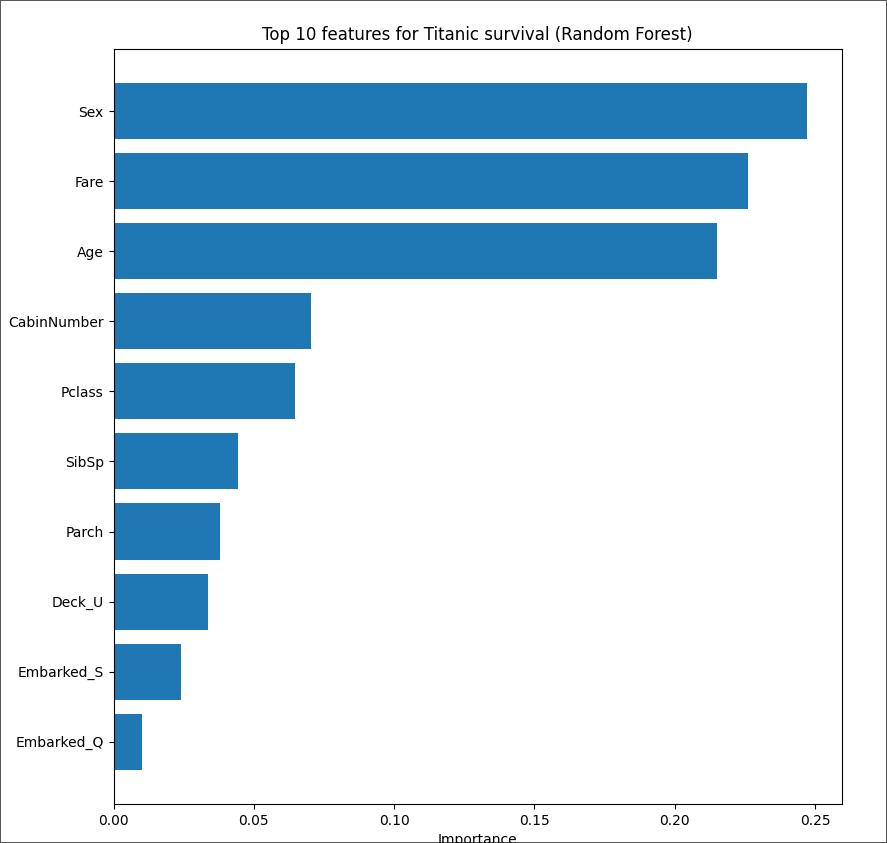
\includegraphics[width=0.78\textwidth]{pic2.png}
    \refstepcounter{figure}
    \caption*{Рисунок \thefigure\ — График с самыми влиятельными признаками}
    \label{fig:important}
\end{figure}

В данной модели наибольшее влияние на результат классификации
оказывают признаки \texttt{Sex}, \texttt{Fare} и \texttt{Age} с влиянием $>= 0.2$.
\texttt{CabinNumber}, \texttt{Pclass} и остальные признаки имеют не такое большое влияние на результат $<= 0.07$.

Это означает, что модель сильно полагается на ограниченное количество признаков.

Отсутствие гладкости предсказаний.

Random Forest формирует решение на основе набора пороговых условий,
что приводит к скачкообразному изменению результата при небольших изменениях входных данных.
Уязвимостью может быть даже незначительное изменение одного признака (например, возраста на 1-2 года)
может изменить путь прохождения по деревьям и привести к противоположному результату классификации.

\section{Атакующие алгоритмы}

Теперь, когда уязвимости известны, нужно выбрать атакующие алгоритмы.

Начну с того, зачем вообще нужно проводить атаку на модель.

Системы машинного обучения в своей основе являются строго зависимыми от данных,
что влечёт за собой ряд существенных последствий. Любые изменения во входных
данных неизбежно отражаются на поведении модели. При этом обучение моделей
машинного обучения осуществляется лишь на ограниченном подмножестве данных —
тренировочном наборе. На этапе эксплуатации модель начинает взаимодействовать с
реальными данными, представляющими генеральную совокупность. Эти данные по
своим статистическим характеристикам могут в целом отличаться от тех, которые
использовались при обучении и тестировании модели. График аппроксимации функции
при наличии подменных данных представлен на рисунке~\ref{fig:approx}.

\begin{figure}[H]
    \centering
    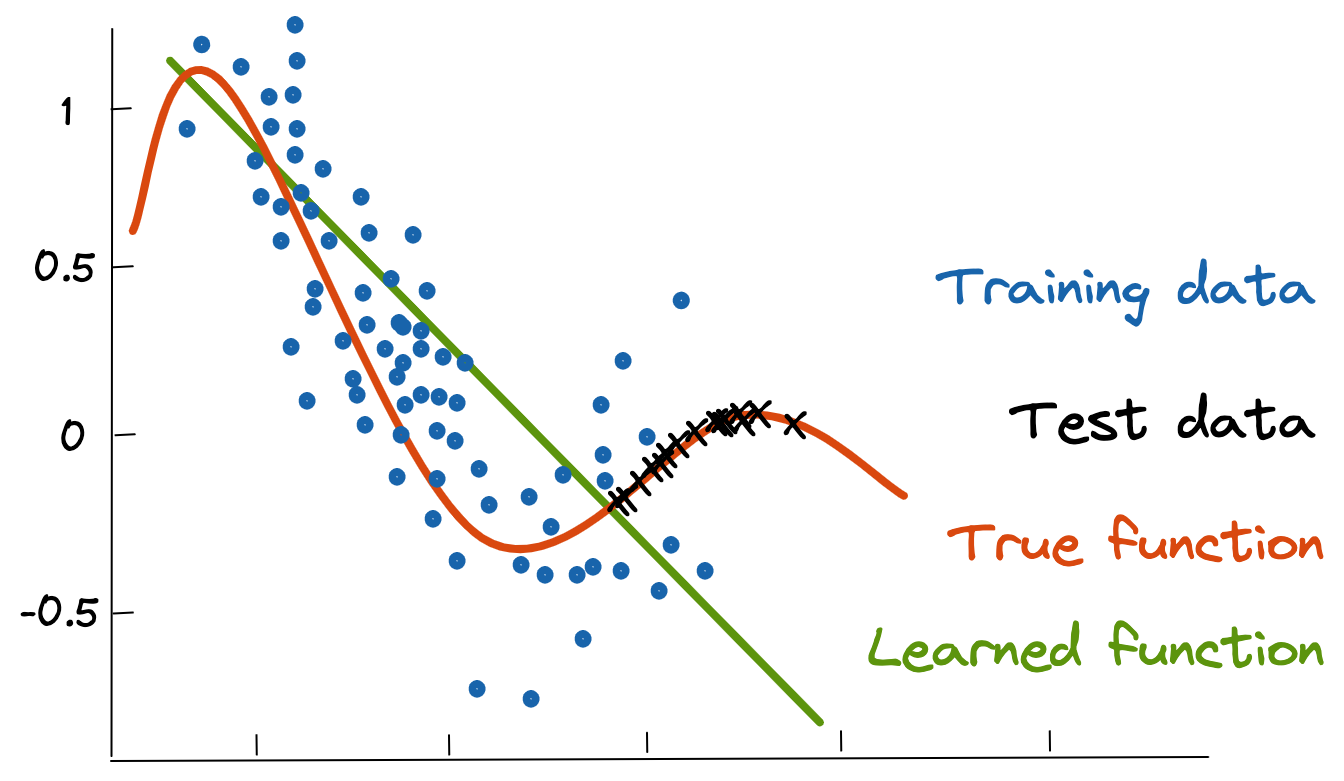
\includegraphics[width=0.78\textwidth]{pic3.png}
    \refstepcounter{figure}
    \caption*{Рисунок \thefigure\ — График аппроксимации функции}
    \label{fig:approx}
\end{figure}

Модель стремится аппроксимировать неизвестную зависимость, изображённую на
графике красной линией. Синим цветом на рисунке обозначены данные
тренировочного набора.

Данные тренировочного набора хорошо обобщаются моделью, и аппроксимирующая
зелёная прямая демонстрирует высокие значения метрик до тех пор, пока реальные
данные сохраняют сходные характеристики с обучающим набором. Однако при
изменении свойств входных данных величина потерь начинает возрастать. Таким
образом, изменение распределения данных напрямую приводит к изменению поведения
модели. При этом такие изменённые данные остаются полностью легитимными для
модели и не выходят за рамки допустимого входного пространства.

Следовательно, в процессе эксплуатации модель машинного обучения может
демонстрировать значения метрик, существенно отличающиеся от достигнутых на
этапе тестирования. На рисунке 3 показан наиболее простой вид расхождения между
реальными и тренировочными данными — ковариантный сдвиг. Вместе с тем
наибольшую опасность для корректной работы модели представляет так называемый
сдвиг концепции, заключающийся в изменении зависимости между входными и
выходными переменными.

Дополнительно возникает вопрос о наличии противоборствующей стороны, которая
целенаправленно подбирает такие входные данные, способные негативно повлиять на
работу модели. Разница между аппроксимирующей прямой и истинной функцией на
рисунке 3 соответствует величине потерь. Поведение функции потерь стандартным
образом определяется её производной по входным данным. Для многомерного
пространства признаков такими характеристиками являются частные производные, а
их совокупность образует якобиан. На рисунке 3 представлена иллюстрация атак
уклонения, основанных на целенаправленных модификациях входных данных, которые
приводят к изменению результата классификации после добавления к корректно
распознаваемому изображению шума, вычисленного с использованием якобиана
функции потерь.

Следует отметить, что подобные модификации входных данных тесно связаны с
проблемой устойчивости моделей машинного обучения. Как правило, алгоритм, в
котором ошибка, присутствующая во входных данных или возникающая в процессе
вычислений, не возрастает или увеличивается незначительно на каждом шаге,
считается устойчивым. В противном случае, когда погрешность существенно
накапливается от шага к шагу, алгоритм классифицируется как неустойчивый. Таким
образом, устойчивость алгоритма представляет собой количественную меру его
чувствительности к изменениям исходных данных. На рисунке~\ref{fig:panda} приведён пример
того, как незначительное изменение входных данных может приводить к
существенному снижению результативности модели.

\begin{figure}[H]
    \centering
    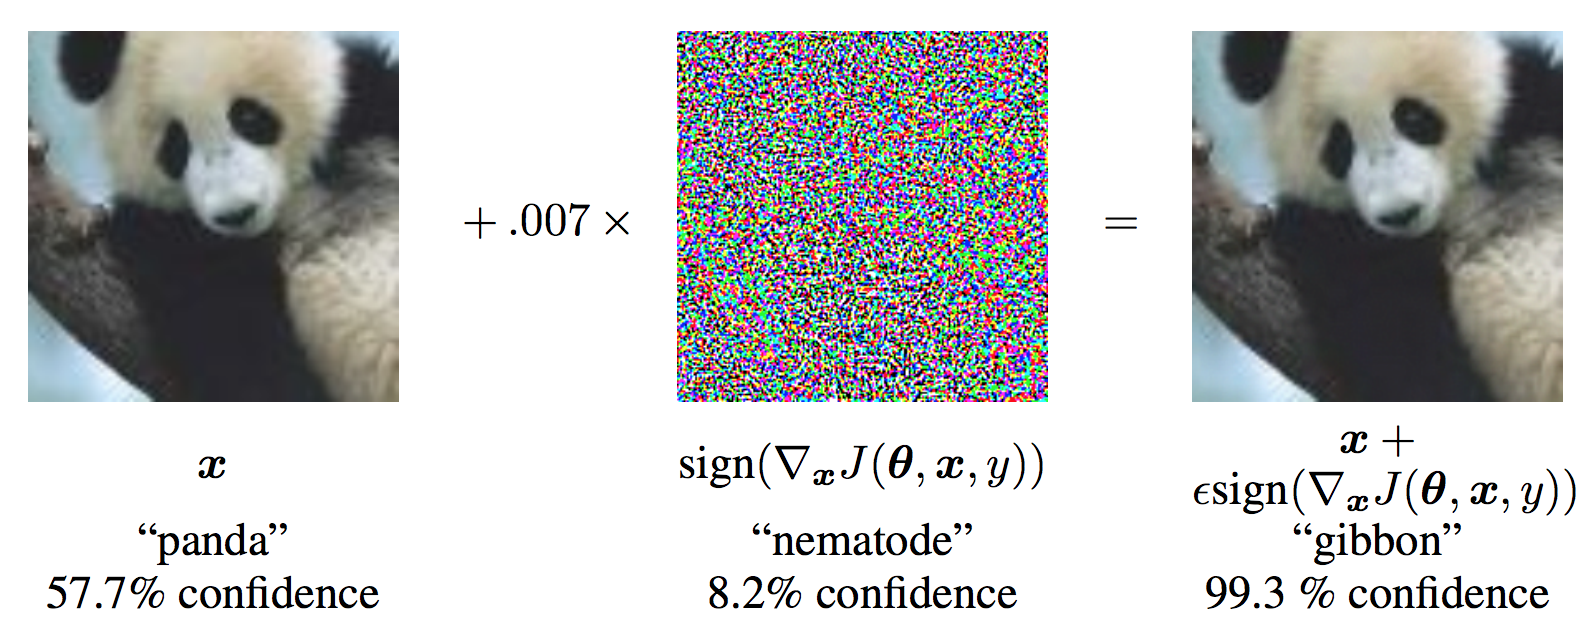
\includegraphics[width=0.78\textwidth]{pic4.png}
    \refstepcounter{figure}
    \caption*{Рисунок \thefigure\ — Враждебная атака с применением шума}
    \label{fig:panda}
\end{figure}

Вот только есть один нюанс. Как упоминалось ранее, модель использует алгоритм Random Forest.
Выражение для предсказания одного дерева в ансамбле Random Forest представлено в формуле~\eqref{eq:tree}.

\begin{equation}
    f_{\text{DT}}(x) = \sum_{k} c_k * 1_{x \in R_k}
    \label{eq:tree}
\end{equation}

\eqexplSetIntro{где:}
\eqexplSetItemWidth{13mm}
\eqexplSetSpace{4mm}
\begin{eqexpl}
    \item{$R_k \subset \R^d$} области признакового пространства, соответствующие листьям дерева,
    \item{$c_k \in [0, 1]$} значение предсказания в листе,
    \item{$1_{x \in R_k}$} индикаторная функция, показывающая, что $x$ попадает в лист $R_k$.
\end{eqexpl}

Данная функция недифференцируема. Для иллюстрации была использована выборка
случайных чисел с дополнительным ограничением $y = x > 30$.
График функции приведён на рисунке~\ref{fig:rf}.

\begin{figure}[H]
    \centering
    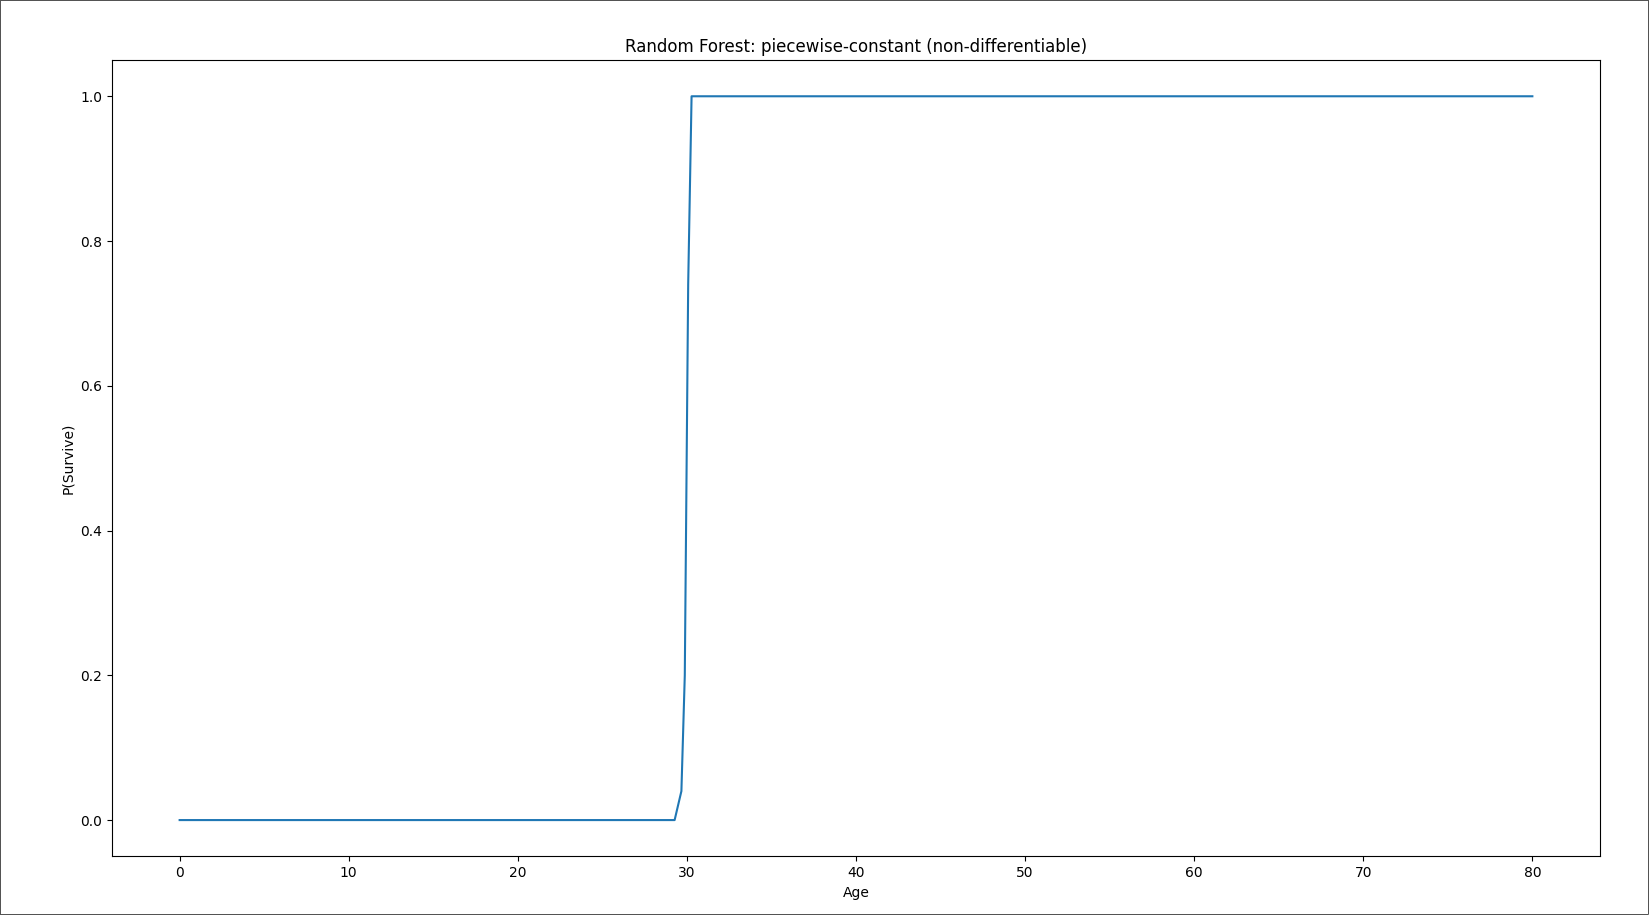
\includegraphics[width=0.78\textwidth]{pic5.png}
    \refstepcounter{figure}
    \caption*{Рисунок \thefigure\ — Предсказание одного дерева Random Forest для $x > 30$}
    \label{fig:rf}
\end{figure}

Поскольку модели на основе деревьев решений недифференцируемы, прямое
вычисление якобиана функции потерь для них невозможно. В связи с этим
используется surrogate-модель на основе нейронной сети, аппроксимирующая
границу решений исходного классификатора. В отличие от Random Forest, нейронная
сеть задаёт гладкую и дифференцируемую функцию, что позволяет вычислять
производные функции потерь по входным признакам и анализировать
чувствительность модели к малым возмущениям входных данных.

\begin{equation}
\mathcal{L}(\theta) = \frac{1}{N} \sum_{i=1}^{N} \big(f_{\text{RF}}(x_i) - \hat{f}_{\text{NN}}(x_i; \theta)\big)^2
\end{equation}

\eqexplSetItemWidth{18mm}
\eqexplSetSpace{4mm}
\begin{eqexpl}
    \item{$f_{\text{RF}}(x)$} предсказание Random Forest,
    \item{$\hat{f}_{\text{NN}}(x; \theta)$} surrogate нейросеть с параметрами $\theta$,
    \item{$\hat{f}_{\text{NN}}(x; \theta)$} градиент surrogate, используемый для оптимизации,
\end{eqexpl}

График функции surrogate-модели нейронной сети представлен на рисунке~\ref{fig:nn}.

\begin{figure}[H]
    \centering
    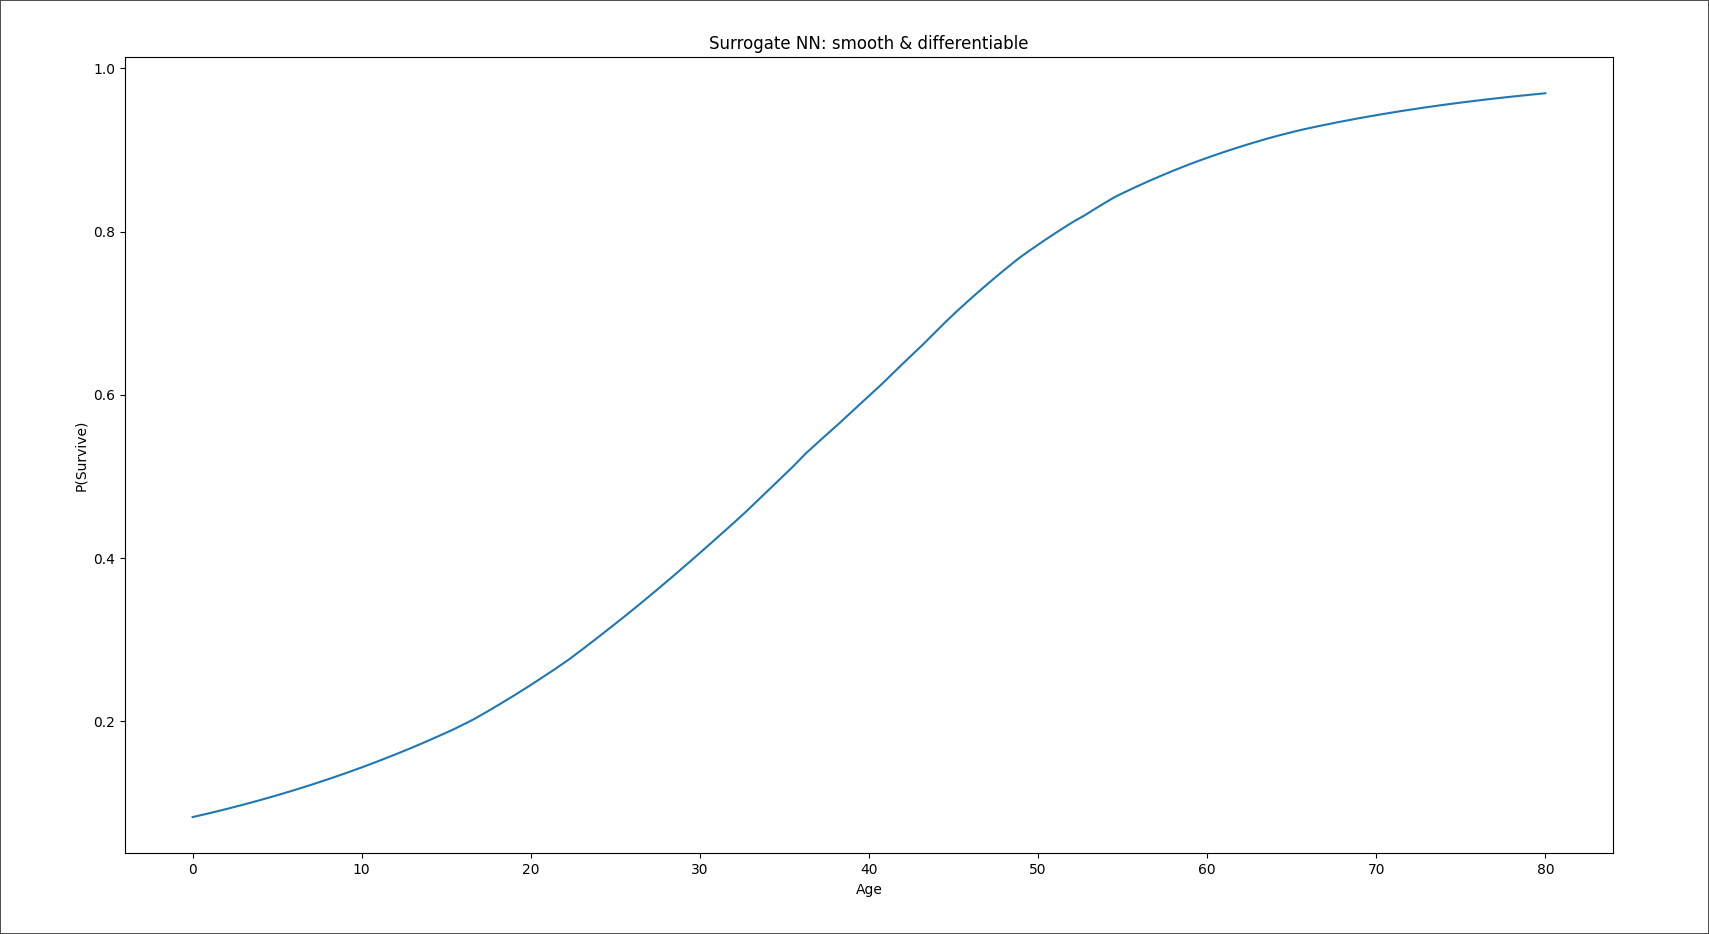
\includegraphics[width=0.78\textwidth]{pic6.png}
    \refstepcounter{figure}
    \caption*{Рисунок \thefigure\ — Предсказание surrogate-модели на основе нейронной сети}
    \label{fig:nn}
\end{figure}

Такое поведение функции можно объяснить тем, что Surrogate NN использует функцию активации.
Функции активации привносят нелинейность в сеть, позволяя ей моделировать сложные структуры данных.
конкретно в моем примере, это функция $ReLU$~\eqref{eq:relu}. А в качестве функции затухания используется $Sigmoid$~\eqref{eq:sigmoid}

\begin{equation}
    ReLU(x) = max(0,x)
    \label{eq:relu}
\end{equation}

\begin{equation}
    \sigma(x) = \frac{1}{1+e^{-x}}
    \label{eq:sigmoid}
\end{equation}

Теперь для выявления характеристик, чувствительность которых основана на якобиане, напишу программу
(см. Приложение 3). Результатом данной программы будет список характеристики с высокой чувствительностью по якобиану для рассматриваемой модели Random Forest.
Выполненная программа представлена на рисунке \ref{fig:sensitive}.

\begin{figure}[H]
    \centering
    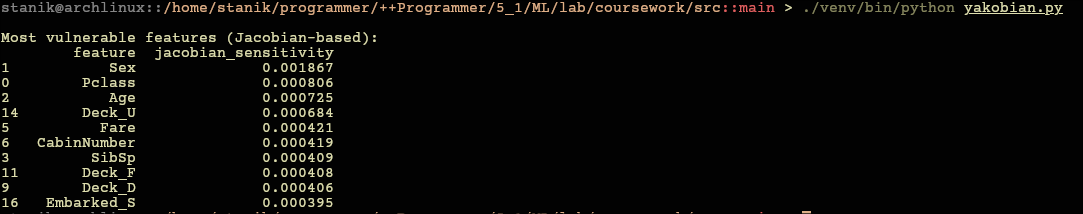
\includegraphics[width=0.78\textwidth]{pic7.png}
    \refstepcounter{figure}
    \caption*{Рисунок \thefigure\ — Характеристики с высокой чувствительностью по якобиану}
    \label{fig:sensitive}
\end{figure}

Для атаки буду использовать алгоритм Surrogate NN. Её цель приближённо учиться
копировать поведение уже обученной модели, конкретно - границу решений: где "выжил" и
где "умер".
В ходе суррогатного моделирования мы строим подменную (или суррогатную) модель
методами машинного обучения для достаточно точной аппроксимации результатов
моделирования. Впоследствии эта обученная статистическая модель может быть
использована для замены исходной компьютерной симуляции.
\[
    \delta Loss / \delta X
\]
В программе я использую 60 эпох

\section{Выводы}

\newpage
\section*{Приложение 1. Код программы}
\begin{verbatim}

import os
import joblib

from sklearn.metrics import accuracy_score, roc_auc_score

from sklearn.ensemble import RandomForestClassifier

from data_preprocessing import get_processed_data

# ---------------------------------------------------------
# Prepare output dir
# ---------------------------------------------------------
os.makedirs("models", exist_ok=True)

# ---------------------------------------------------------
# Load data
# ---------------------------------------------------------
X_train, X_val, y_train, y_val, df, scaler = get_processed_data(
    data_dir="titanic/", test_size=0.2, random_state=42
)

X_train_scaled = scaler.fit_transform(X_train)
X_val_scaled = scaler.transform(X_val)

# Save scaler
joblib.dump(scaler, "models/scaler.pkl")


# ============================================================
# Random Forest
# ============================================================
rf = RandomForestClassifier(n_estimators=400, random_state=42)
rf.fit(X_train, y_train)

pred_rf = rf.predict(X_val)
proba_rf = rf.predict_proba(X_val)[:, 1]

print("=== Random Forest ===")
print("Acc:", accuracy_score(y_val, pred_rf))
print("AUC:", roc_auc_score(y_val, proba_rf))
print()

joblib.dump(rf, "models/random_forest.pkl")


\end{verbatim}

\end{document}
